%!TEX root = ../main.tex

\section{Results}
\label{s:results}

\subsection{Fake versus real normals}
	\todo[inline]{Show results of PN triangles with fake and real normals, and discuss differences}
	\todo[inline]{Computational complexity of the fake normals and the real normals, consider one triangle.}
	\todo[inline]{Any unsolved problems?}

\iftoggle{PHONG}{
\subsection{Phong tesselation versus PN triangles}
	\future{Show comparison of Phong tesselation with PN triangles: performance, visual results, continuity, probably in cooperation with Jelle and Gerben}
	\future{Any unsolved problems?}
}

\begin{figure}
	\centering
	\begin{subfigure}{0.5\columnwidth}
		\centering
		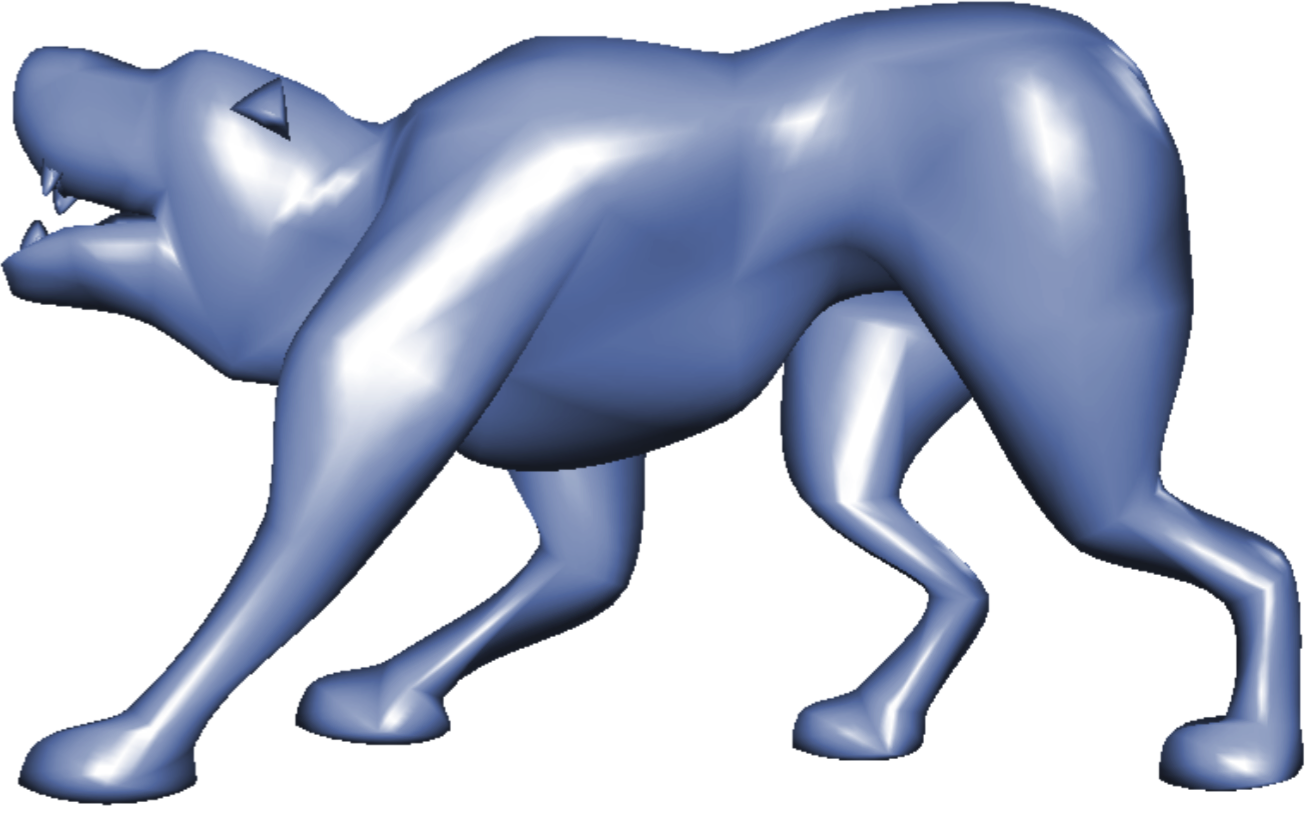
\includegraphics[width=\textwidth]{content/img/results/dogCPU.png}
		\caption{CPU}
		\label{fig:results:cpugpu:cpu}
	\end{subfigure}
	\begin{subfigure}{0.5\columnwidth}
		\centering
		% \includegraphics[width=\textwidth]{./img/_}
		\missingfigure[figwidth=\textwidth]{The dog rendered with our code}
		\caption{GPU}
		\label{fig:results:cpugpu:gpu}
	\end{subfigure}	
	\caption{A game character \subref{fig:results:cpugpu:cpu} rendered on the CPU by \citeauthor{vlachos2001curved} and \subref{fig:results:cpugpu:gpu} on the GPU by our implementation.}
	\label{fig:results:cpugpu}
\end{figure}

\subsection{Pipeline}
	\Cref{fig:results:cpugpu} shows the rendering by \citeauthor{vlachos2001curved} next to our rendering of, probably, the same model. The only difference between these two models should be the pattern in which the triangles of the input mesh are subdivided into flat triangles. \todo{A visual inspection of the models shows no differences between the two models.}